\documentclass[../../main.tex]{subfiles}
\begin{document}
{\bf[解]}

与えられた関数
\begin{align}
  f(x) = (x^2-4)(x^2-9) = (x+2)(x-2)(x+3)(x-3) \label{eq:1}
\end{align}
について考える．一階微分は
\begin{align}
  f'(x)=2x(2x^2-13) \label{eq:2}
\end{align}
である．よって$f(x)$の増減表は以下のようになる．

\begin{table}[htb]
  \centering
  \caption{$f(x)$ の増減表}
  \renewcommand{\arraystretch}{1.3}
  \begin{tabular}{c|ccccccc}
    $x$ & $\cdots$ & $-\sqrt{\dfrac{13}{2}}$ & $\cdots$ & $0$ & $\cdots$ & $\sqrt{\dfrac{13}{2}}$ & $\cdots$ \\
    \hline
    $f'(x)$ & $-$ & $0$ & $+$ & $0$ & $-$ & $0$ & $+$ \\
    \hline
    $f(x)$ & $\searrow$ & 極小 & $\nearrow$ & 極大 & $\searrow$ & 極小 & $\nearrow$ \\
    &            & $-\dfrac{25}{4}$ &    & $36$ &            & $-\dfrac{25}{4}$ &
  \end{tabular}
\end{table}

従って$y=f(x)$のグラフの概形は以下のようになる．

\begin{figure}[htb]
  \centering
  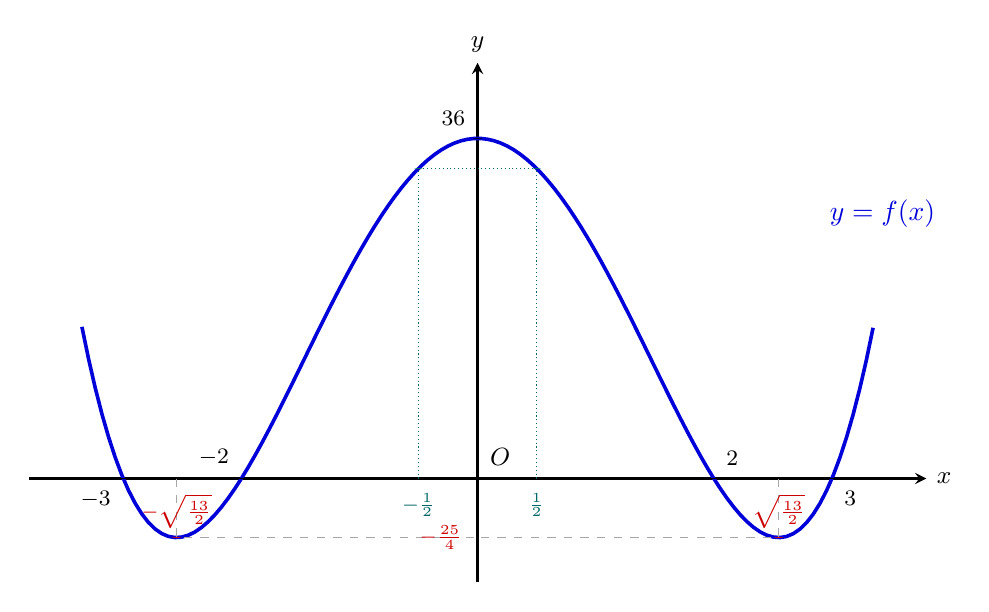
\begin{tikzpicture}[
      xscale=1.5,
      yscale=0.12,
      >=stealth,
      every node/.style={font=\small}
    ]

    % --- 1. 定数・極値の定義 ---
    % 極小値をとる x = sqrt(13/2) ≈ 2.5495
    % 極小値 y = -25/4 = -6.25
    \def\xMin{2.5495}
    \def\yMin{-6.25}

    % 代表点 x = 1/2 のときの値: f(1/2) = (1/4 - 4)(1/4 - 9) = (-15/4)*(-35/4) = 525/16 = 32.8125
    \def\xRef{0.5}
    \def\yRef{32.8125}

    % --- 2. 座標軸 ---
    \draw[->, thick] (-3.8, 0) -- (3.8, 0) node[right] {$x$};
    \draw[->, thick] (0, -11) -- (0, 44) node[above] {$y$};
    \node[above right=1pt] at (0, 0) {$O$};

    % --- 3. グラフ y = f(x) の描画 ---
    % f(x) = x^4 - 13x^2 + 36
    \draw[line width=1.3pt, blue!85!black, domain=-3.35:3.35, samples=120]
    plot (\x, {\x*\x*\x*\x - 13*\x*\x + 36});
    \node[blue!85!black, font=\normalsize\bfseries, right] at (2.9, 28) {$y = f(x)$};

    % --- 4. 切片および主要点のプロット ---
    % x 切片 (±3, 0), (±2, 0)
    \fill (-3, 0) circle (1.2pt);
    \node[below left=1pt, font=\footnotesize] at (-3, 0) {$-3$};

    \fill (-2, 0) circle (1.2pt);
    \node[above left=1pt, font=\footnotesize] at (-2, 0) {$-2$};

    \fill (2, 0) circle (1.2pt);
    \node[above right=1pt, font=\footnotesize] at (2, 0) {$2$};

    \fill (3, 0) circle (1.2pt);
    \node[below right=1pt, font=\footnotesize] at (3, 0) {$3$};

    % y 切片 (0, 36) (極大値)
    \fill (0, 36) circle (1.2pt);
    \node[above left=1pt, font=\footnotesize] at (0, 36) {$36$};

    % --- 5. 極小値の補助線 ---
    % x = sqrt(13/2)
    \draw[dashed, gray!70] (\xMin, 0) -- (\xMin, \yMin) -- (0, \yMin);
    \fill[red!80!black] (\xMin, \yMin) circle (1.2pt);
    \node[below=2pt, font=\scriptsize, red!80!black] at (\xMin, 0) {$\sqrt{\frac{13}{2}}$};

    % x = -sqrt(13/2)
    \draw[dashed, gray!70] (-\xMin, 0) -- (-\xMin, \yMin) -- (0, \yMin);
    \fill[red!80!black] (-\xMin, \yMin) circle (1.2pt);
    \node[below=2pt, font=\scriptsize, red!80!black] at (-\xMin, 0) {$-\sqrt{\frac{13}{2}}$};

    \node[left=2pt, font=\scriptsize, red!80!black] at (0, \yMin) {$-\frac{25}{4}$};

    % --- 6. 代表点 x = ±1/2 への射影（解の議論用） ---
    \draw[densely dotted, teal!80!black] (\xRef, 0) -- (\xRef, \yRef) -- (-\xRef, \yRef);
    \draw[densely dotted, teal!80!black] (-\xRef, 0) -- (-\xRef, \yRef);
    \fill[teal!80!black] (\xRef, \yRef) circle (1.0pt);
    \fill[teal!80!black] (-\xRef, \yRef) circle (1.0pt);
    \node[below=2pt, font=\scriptsize, teal!80!black] at (\xRef, 0) {$\frac{1}{2}$};
    \node[below=2pt, font=\scriptsize, teal!80!black] at (-\xRef, 0) {$-\frac{1}{2}$};

  \end{tikzpicture}
  \caption{$y = f(x) = (x^2 - 4)(x^2 - 9)$ のグラフ}
  \label{fig:graph_f_quartic}
\end{figure}

さて$g(t)$について考えるために，$f(t)=f(t+1)$を考えると
\begin{align}
  &f(t)\le f(t+1) \\
  \Longleftrightarrow
  &(t+3)(t-1)(t+4)(t-2) \le (t+2)(t-2)(t+3)(t-3) \\
  \Longleftrightarrow
  &(t+3)(t-2)\left[t^2+3t-4-(t^2-t-6)\right] \le 0 \\
  \Longleftrightarrow
  &(t+3)(t-2)(4t+2)\le 0
\end{align}
である．従って，$f(t)\le f(t+1)$となるのは
\begin{align}
  -3 \le t \le \dfrac{-1}{2}, 2 \le t
\end{align}
である．
従って，$y=f(t)$のグラフの概形と合わせて求める関数$g(x)$は以下のようになる．
\begin{align}
  g(x)=\left\{
    \begin{array}{ll}
      f(t+1)&(-3\le t\le -1) \\
      36    &(-1\le t\le 0) \\
      f(t)    &(0\le t\le 2) \\
      f(t+1)&(2\le t\le 3)
    \end{array}
    \right.
  \end{align}
  これを図示すると下図である．$\cdots$(答)

  \begin{figure}[htb]
    \centering
    \begin{tikzpicture}[
        xscale=1.5,
        yscale=0.08,
        >=stealth,
        every node/.style={font=\small}
      ]

      % --- 1. 関数マクロの定義 ---
      % f(t) = t^4 - 13t^2 + 36
      % f(t+1) = t^4 + 4t^3 - 7t^2 - 22t + 24
      \def\FuncF#1{(#1)^4 - 13*(#1)^2 + 36}
      \def\FuncG#1{(#1)^4 + 4*(#1)^3 - 7*(#1)^2 - 22*(#1) + 24}

      % --- 2. 座標軸 ---
      \draw[->, thick] (-3.8, 0) -- (3.8, 0) node[right] {$t$};
      \draw[->, thick] (0, -10) -- (0, 100) node[above] {$y$};
      \node[below left=2pt] at (0, 0) {$O$};

      % --- 3. 背景の参考曲線（薄い破線） ---
      % f(t) の全体軌跡
      \draw[thin, dashed, gray!60, domain=-3.3:3.3, samples=80]
      plot (\x, {\FuncF{\x}});
      \node[gray!70!black, font=\scriptsize, right] at (3.1, 40) {$y = f(t)$};

      % f(t+1) の全体軌跡
      \draw[thin, dashed, gray!60, domain=-3.3:2.2, samples=80]
      plot (\x, {\FuncG{\x}});
      \node[gray!70!black, font=\scriptsize, left] at (-3.2, 40) {$y = f(t+1)$};

      % --- 4. g(t) のグラフ本体（太線実線） ---
      % (i) -3 <= t <= -1 : f(t+1) (t=-3 で 0, t=-1 で 36)
      \draw[line width=1.5pt, blue!85!black, domain=-3:-1, samples=60]
      plot (\x, {\FuncG{\x}});

      % (ii) -1 <= t <= 0 : 定数 36
      \draw[line width=1.5pt, blue!85!black] (-1, 36) -- (0, 36);

      % (iii) 0 <= t <= 2 : f(t) (t=0 で 36, t=2 で 0)
      \draw[line width=1.5pt, blue!85!black, domain=0:2, samples=60]
      plot (\x, {\FuncF{\x}});

      % (iv) 2 <= t <= 3 : f(t+1) (t=2 で 0, t=3 で 60)
      \draw[line width=1.5pt, blue!85!black, domain=2:3, samples=60]
      plot (\x, {\FuncG{\x}});

      % グラフ名ラベル
      \node[blue!85!black, font=\normalsize\bfseries, right] at (2.4, 52) {$y = g(t)$};

      % --- 5. 区間の境界点・補助線 ---
      % t = -3 (y = 0)
      \fill (-3, 0) circle (1.2pt);
      \node[below=2pt, font=\footnotesize] at (-3, 0) {$-3$};

      % t = -1 (y = 36)
      \draw[dashed, gray!70] (-1, 0) -- (-1, 36);
      \fill[blue!85!black] (-1, 36) circle (1.2pt);
      \node[below=2pt, font=\footnotesize] at (-1, 0) {$-1$};

      % t = 0 (y = 36)
      \fill[blue!85!black] (0, 36) circle (1.2pt);
      \draw[dashed, gray!70] (-1, 36) -- (0, 36);
      \node[left=2pt, font=\footnotesize] at (0, 36) {$36$};

      % t = 2 (y = 0)
      \fill[blue!85!black] (2, 0) circle (1.2pt);
      \node[below=2pt, font=\footnotesize] at (2, 0) {$2$};

      % t = 3 (y = f(4) = (16-4)(16-9) = 12*7 = 84 / f(t+1)|_{t=3} = 60)
      \pgfmathsetmacro{\yAtThree}{\FuncG{3.0}}
      \draw[dashed, gray!70] (3, 0) -- (3, \yAtThree) -- (0, \yAtThree);
      \fill[blue!85!black] (3, \yAtThree) circle (1.2pt);
      \fill (3, 0) circle (1.2pt);
      \node[below=2pt, font=\footnotesize] at (3, 0) {$3$};
      \node[left=2pt, font=\footnotesize] at (0, \yAtThree) {$84$};

      % --- 6. 区間ごとの関数表示（注釈） ---
      \node[teal!85!black, font=\scriptsize, align=center] at (-2.1, 15) {$f(t+1)$};
      \node[purple!85!black, font=\scriptsize, align=center] at (-0.5, 42) {$36$};
      \node[teal!85!black, font=\scriptsize, align=center] at (1.0, 15) {$f(t)$};
      \node[teal!85!black, font=\scriptsize, align=center] at (2.9, 20) {$f(t+1)$};

    \end{tikzpicture}
    \caption{関数 $y = g(t)$ のグラフ（青実線部，$-3 \leqq t \leqq 3$）}
    \label{fig:graph_gt}
  \end{figure}

  \newpage
  \end{document}
